\documentclass[11pt]{article}
\usepackage[utf8]{inputenc}
\usepackage{graphicx}
\usepackage{caption}
\usepackage{subcaption}
\usepackage{booktabs}
\usepackage[margin=0.5in]{geometry} % Set all margins to 1 inch



\begin{document}

% \title{TP 4}
% \author{Mahdi Moghadasi \\ 20184188 \and Ibrahim Ould Saada \\ 20151421}
% \date{}
% \maketitle
\noindent \textbf{TP 4} \hfill \textbf{Mahdi Moghadasi (20184188), Ibrahim Ould Saada (20151421)}

\section{Tests boite noire}

Les hypothèses :
\begin{itemize}
    \item Les méthodes doivent rejeter les paires de devises non valides et fournir un message d'erreur ou une exception.
    \item Pour les montants non valides, les méthodes doivent soit lever une exception, soit renvoyer un message d'erreur spécifique, indiquant que le montant saisi est en dehors de la plage acceptable.
    \item Nous avons assumer que nous pouvons le arraylist par défaut fourni dans le code pour faire les tests qui se initialise en appelant la méthode Currency.init().
    \item nous avons remarquer que les test fait avec les nom donner en spécification("EUR","USD" ,...) ne donnait rien ce qui montre un écart entre le nom de la spécification et le nom attendu en entré par la méthode, nous avons donc assumer qu'il fallait fournir des test avec les nom attendu par la méthode ("Euro", "US Dollar", ...) pour vérifier si la validité des devise elle même était respecter
\end{itemize}

Dans cette partie, pour choisir les cas de tests, nous avons utilisé les approches de partition du domaine des entrées en classes d’équivalence et analyse des valeurs frontières.


\subsection{Méthode currencyConverter.Currency.convert()}
\subsubsection{Méthodologie}

Cette méthode prend deux arguments \texttt{(Double amount, Double exchangeValue)}.
Nous avons choisi les classes d'équivalence pour \texttt{amount} comme suit :

    \hspace{-7mm}
    - D1 : \{(\texttt{amount}) $|$ \texttt{amount} $<$ 0\} \\
    - D2 : \{(\texttt{amount}) $|$ $0 \leq \texttt{amount} \leq 1,000,000$\} \\
    - D3 : \{(\texttt{amount}) $|$ \texttt{amount} $>$ 1,000,000\} \\
    
Les valeurs frontières de  \texttt{amount} sont : $-1$, $0$, $1,000,000$, $1,000,001$. \\

Nous avons choisi les classes d'équivalence pour \texttt{exchangeValue} comme suit :

    \hspace{-7mm}
    - D1 : \{(\texttt{exchangeValue}) $|$ \texttt{exchangeValue} $\leq 0$\} \\
    - D2 : \{(\texttt{exchangeValue}) $|$ \texttt{exchangeValue} $>$  0\} \\

Les valeurs frontières de \texttt{exchangeValue} sont : $-1$, $0$, $1$. \\
    
\subsubsection{Résultats}

Pour nos 2 paramétrées, nous avons observe que la classe d'équivalence valide(D2) passe les tests. Pourtant, pour les valeurs invalides, la méthode ne lance pas une exception \textit{IllegalArgumentException}.
Pour cette raison, ces tests échoues.


\subsubsection{Observations}
Nous avons constaté grâces aux résultat des test que toutes les valeurs des paramètres sont acceptées, ce qui ne devrait pas être le cas car ça ne respecte pas nos spécifications définies pour les tests blackbox.




\subsection{Méthode currencyConverter.MainWindow.convert()}

\subsubsection{Méthodologie}

Cette méthode prend 4 arguments : \texttt{(String currency1, String currency2, ArrayList<Currency> currencies, Double amount)}. Nous avons choisi les classes d'équivalence pour \texttt{currency} comme suit : \\

    \hspace{-7mm}
    - D1 : \{(currency) | currency est dans la liste currencies d'énoncé valide)\} \\
    - D2 : \{(currency) | currency n'est pas dans la liste currencies d'énoncé(invalide)\} \\

Pour \texttt{amount}, nous avons défini les classes d'équivalence suivantes : \\
    \hspace{-7mm}
    - D1 : \{(amount) | amount < 0\} \\
    - D2 : \{(amount) | 0$ \leq$ amount$ \leq $1 000 000\} \\
    - D3 : \{(amount) | amount > 1 000 000\} \\


\subsubsection{Résultats}
Comme pour la méthodes précédentes, les résultats des tests nous indiquent que la méthode accepte toutes les valeurs du paramètres amount, currency1 et currency2. La méthode ne lance pas aucune Exceptions quand elle reçoit des valeurs non-valide. La méthode ne passe pas plusieurs tests et respecte pas les spécifications.


\subsubsection{Observations}
-Dans notre cas nous avons remarqué qu'il faut tout d'abord comprendre la structure  de arraylist currencies créer des test pertinent, bien que ça éloigne un peu du concept de black box(gray box). \\

-les currencies CAD et AUD ne sont pas prise en charge par le arraylist par défaut de l'application et elle retourne 0.0 pour ces devises, ce qui n'est pas une bonne pratique de programmation.




\section{Tests boite blanc}

Veuillez referez vous a la fin du rapport en page 4 pour voir les graphes de flot de contrôle. Pour voir les images plus clairement, vous pouvez vous référer au répertoire git dans le chemin \texttt{tp4/analyse/CFD/}.


\subsection{\textbf{Méthode currencyConverter.MainWindow.convert()}}
Pour les tests boite blanche de cette méthode, nous avons considéré les degrés de couvertures suivant:
1. Couverture des conditions (et des arcs) \\
2. Couverture des chemins indépendants \\
3. Couverture des i-chemins\\

\subsubsection{Méthodologie}
% Les classe d'equivalence comme suit:
% \begin{itemize}
%     \item D4 {arraylist valide}
%     \item D5 {arraylist vide}
%     \item D6 {arraylist non vide mais sans exchange values}
% \end{itemize}
% de cette manière tout les chemin lié aux if statement  et aux for loop sont couvert.
% le premier et le deuxième if statement dans le code sont géré par la validité de currency2.

% Le troisième if statement quant a lui est géré par la validité de currency1

% Les jeux de test que nous avons utilisé sont :

% \begin{itemize}
%     \item T1 ${"US Dollar", "Euro"}$
%     \item T2 {"Invalid", "Euro"}
%     \item T3 {"Euro","Invalid"}
%     \item T3 {current.init()}
%     \item T4 {empty array list}
%     \item T5 {arraylst no exchange}
% \end{itemize}

\textbf{\textit{1. Couverture des conditions (et des arcs):}} Puisque nous n'avons pas de condition composé dans cette méthode, Couverture des conditions (et des arcs) se réduit à l'analyse de couverture des arcs. puisque notre analyse des Couverture des chemins indépendants couvre aussi l'analyse de couverture des arcs, nous pouvons maintenant passer a cette analyse. \\
\textbf{\textit{2. Couverture des chemins indépendants:}} Pour cette analyse, nous avons observé notre graphe de flux de contrôle et trouver tous les chemins( 16 chemins). Après, nous avons trouvé tous les chemins qui sont faisable selon la logique du code( 6 chemins). Nous avons formé une matrice en convertissant ces chemins en leurs représentation vectorielle. Avec l'aide d'algèbre linéaire, nous avons éliminer les ligne dépendante linéairement pour nous retrouver avec 4 chemins indépendants. (Les calcules se trouve dans \texttt{TP4/analyse/analyse-independant-paths.ipynb}. Nous avons écrit les tests selon ces chemins. Voici les 4 chemins et les méthodes de tests qui les couvres:

\hspace{-6mm}
-1 2 3 4 5 6 7 8 9 10 11 12 13 14  \hfill testSingleCurrencyInList() \\
-1 2 3 4 8 14                     \hfill  testConvertWithEmptyCurrenciesList() \\      
-1 2 3 4 5 4 8 14                \hfill   testSingleCurrency2NotFound() \\
-1 2 3 4 5 6 7 8 9 10 9 14       \hfill   testSingleCurrency1NotFound() \\


\textbf{\textit{3. Couverture des i-chemins:}} Pour cette analyse, nous allons considérer tous les chemins faisable selon la logique du code. Nous avons écrit les tests selon ces chemins. Dans la méthode, nous avons deux boucle for simple qui itère en fonction de la taille de arrayList \texttt{currencies}. Puisqu'il ne sont pas dépendant  et qu'il ne sont pas imbriqué, c'est facile de les testes en donnant les arrayLists ayant les tailles différentes.  Voici les 6 i-chemins et les méthodes de tests qui les couvres: \\ 

\hspace{-6mm}
-1 2 3 4 5 6 7 8 9 10 11 12 13 14  \hfill testSingleCurrencyInList() \\
-1 2 3 4 8 14                   \hfill    testConvertWithEmptyCurrenciesList() \\      
-1 2 3 4 i(5 4) 8 14            \hfill    testCurrency2NotFound() \\
-1 2 3 i(4 5) 6 7 8 9 i(10 9) 14 \hfill     testCurrency1NotFound() \\
-1 2 3 i(4 5) 6 7 8 9 10 11 12 13 14 \hfill testcurrenciesFound() \\
-1 2 3 i(4 5) 6 7 8 i(9 10) 11 12 13 14 \hfill testcurrenciesFound() \\ 

\textit{ici le i signifie le nombre de fois ou on va boucler sur les noeuds entre parenthèses et ce nombre dépend de l'emplacement de currency1 et currency2 dans l'arraylist(l'effet des break)}

\subsubsection{Résultats}
Le test  pour testSingleCurrencyInList() passe. \\
Pour testConvertWithEmptyCurrenciesList(), testSingleCurrency2NotFound(), testSingleCurrency1NotFound(), on s'attend a avoir un illegalargumentException mais on n'a aucune Exception qui se lance et a la place ça nous renvoies 0.0 comme valeur, ce qui n'est pas acceptable. Les tests testTenCurrencyConversionValid(), testTenCurrencyConversion1NotFound() testTenCurrencyConversion2NotFound() ont comme but de tester plusieurs itération de boucle for et donc tester les i-chemin. comme les autres tests, la méthode passe pour les valeurs valides mais elle ne lance pas d'exceptions quand la valeur de paramètre est invalide.

\subsubsection{Observation}
% On observe aussi que peut importe le nombre de boucle dans les i-chemin le résultats ne change pas
Dans notre fichier \texttt{test/MainWindowWhiteBoxTest.java} nous avons plusieurs tests qui ne sont pas indiqué dans la partie méthodologie comme testConversionFromUSDToVariousCurrenciesUsingLiterals. Cette méthode teste la logique du programme et puisque le teste ne passe pas, on a appris que le code utilise == pour la comparaison des strings. (au lieu de methode .equals()), ce qui empêche la méthode de conversion de trouver la devise correspondante dans ces cas. \\

Nous constatons par les tests \texttt{testNullCurrency1InValid} et \texttt{testNullCurrency2InValid} que si les strings sont données comme null, il n'y a aucune exception qui se lance a la place de NullPointerException attendue. \\

Nous avons aussi observé que la méthode prend le type \texttt{Double} pour l'argument amount. Ce choix de type peut causer des problèmes au différents niveau comme performance et doit être justifier si nous voulons retourner null comme la valuer de amount pour les cas spécifiques. De toute façon, ce n'est pas le cas avec le code.

\subsection{Méthode currencyConverter.Currency.convert()}
\subsubsection{Méthodologie}
Pour cette méthode nous avons remarqué qu'elle est extrêmement simple et n'emprunte qu'un seul chemin direct sans des conditions. Donc pour cette méthode, nous nous somme dit que nous allons choisir la couverture des arc comme degré de couverture, ce qui peut se réduire a une couverture des instructions.
pour cela nous avons pris un jeu de tests  où le premier élément correspond a \texttt{amount} et le deuxième a \texttt{exchangeValue}

voici quelques éléments pertinents de notre jeu de test:
    \hspace{-7mm}
    - T1 : \{(-1,1.2)\} \\
    - T2 : \{(100,1.2)\} \\
    - T3 : \{(1 000 001,1.2)\} \\
    - T4 : \{(0,1.2)\} \\
    - T5 : \{(1000000,1.2)\} \\
    - T6 : \{(null,null)\} \\
    

\subsubsection{Résultats}
Le jeu de test T2 passe sans problème. Nous voyons que les tests ne lance pas d'exception alors que nous attendions un illegalArgumentException pour les jeux de test T1 et T3. Comme vu avant, cette méthode donne les bons résultats pour les arguments valides mais elle ne lance pas d'exceptions pour les arguments invalide.


\subsubsection{Observation}
Nous avons observé que cette methode lance bien l'exception NullPointerException quand les arguments données sont null.



\begin{figure}[h]
    \centering
    \begin{minipage}{0.6\textwidth}
        \centering
        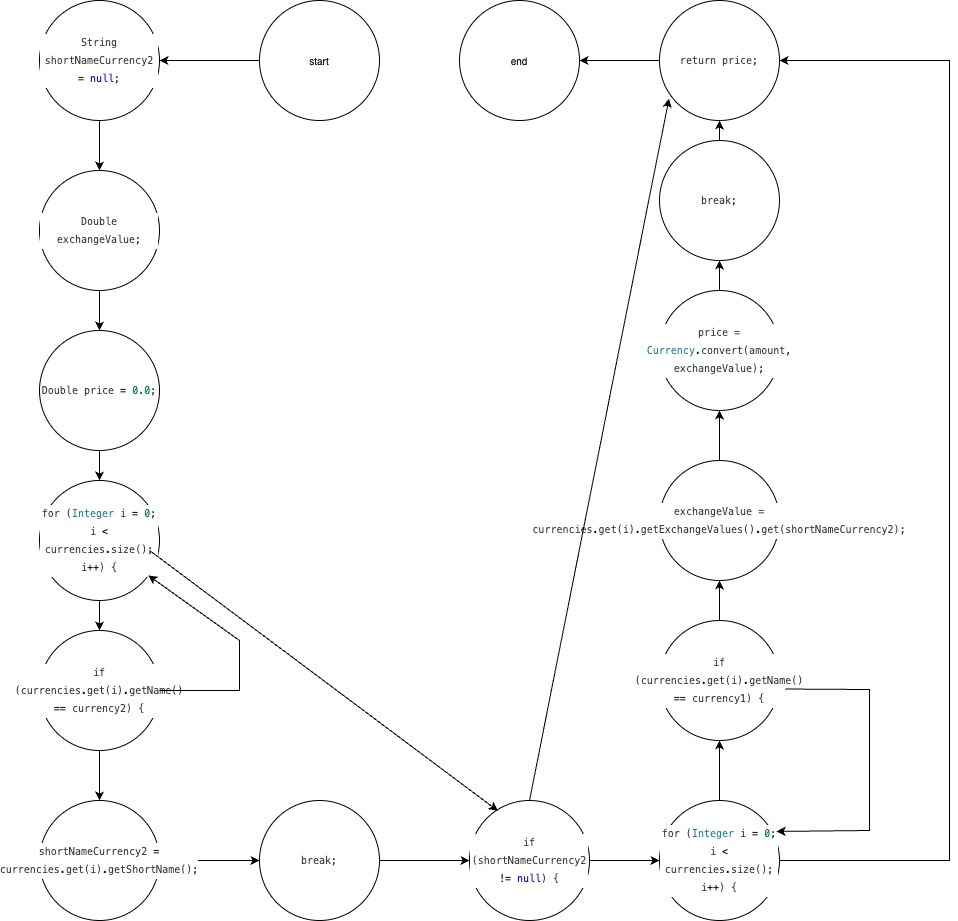
\includegraphics[width=0.9\linewidth]{MainWindow.convert()-no code.jpg}
        \caption{MainWindow.convert() CFG}
    \end{minipage}\hfill
    \begin{minipage}{0.4\textwidth}
        \centering
        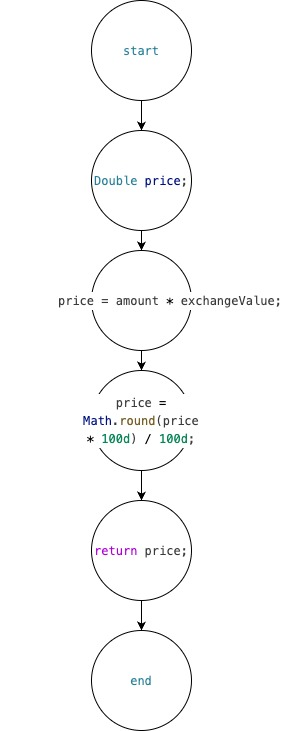
\includegraphics[width=0.4\linewidth, angle=90]{Currency.convert()-no code.jpg}
        \caption{Currency.convert() CFG}
    \end{minipage}
\end{figure}


\end{document}